\chapter{Introduction to Machine Learning}
	初めて機械学習という単語を聞いた人は 『機械学習 = 人工知能』 と間違えるかもしれませんが、
	機械学習とは人工知能を作るための数多あるアプローチのうちの1つで、簡単に言うと、
	『データから自動的に学んで予測・分類などを行う仕組み』
	\cite{essence_of_ML}とされます。
	そして、機械学習は一般的に次の3つに分けられます。
	
	\section{機械学習の分類}
		\begin{itemize}
			\item 教師ある学習 (Supervised Learning)
			\item 教師なし学習 (Unsupervised Learning)
			\item 強化学習 (Reinforcement Learning)
		\end{itemize}
		
		それぞれ、教師あり学習はデータと答えのセットを人間が用意し、
		データが与えられたら正しい答えが出力される様に学習される手法です。
		
		教師なし学習は、データのみを与え
		その中から法則性やパターン、類似性を抽出される手法です。
		
		最後に強化学習は、エージェントと呼ばれる物を用意し、
		それが行動した結果得られる報酬を最大化するように
		エージェントを学習させる手法です。
	
	\newpage
	\section{k近傍法}
		ここでは、k近傍法(以下、kNN)を使って機械学習を体験してみましょう。
		ちなみに、kNNは教師あり学習に分類されます。\\
		
		kNNのアルゴリズムは次の通りです。\cite{python_ML_pro}
		\begin{itemize}
			\item kの値と距離指標を選択する。
			\item 分類したいサンプルからk個の最近傍のデータ点を見つけ出す。
			\item 多数決によりクラスラベルを割り当てる。
		\end{itemize}
		
		詳細な図は教科書 P.11を参照して下さい。
	
	\section{kNNの学習}
		では、早速Google Colab上でkNNを実際に動かしてみましょう。
		なお、以下のコードで\texttt{matplotlib}、\texttt{sklearn}、\texttt{mlxtend}を利用しています。
		Google Colabでは事前にこれらのライブラリがインストールされていますが、
		それ以外の環境では、次のコマンドを実行することによりインストールする事が可能です。\\
		
		\begin{framed}
			\texttt{pip install ライブラリ名} \\
			\\ \
			例) \texttt{pip install torch}
		\end{framed}


		
		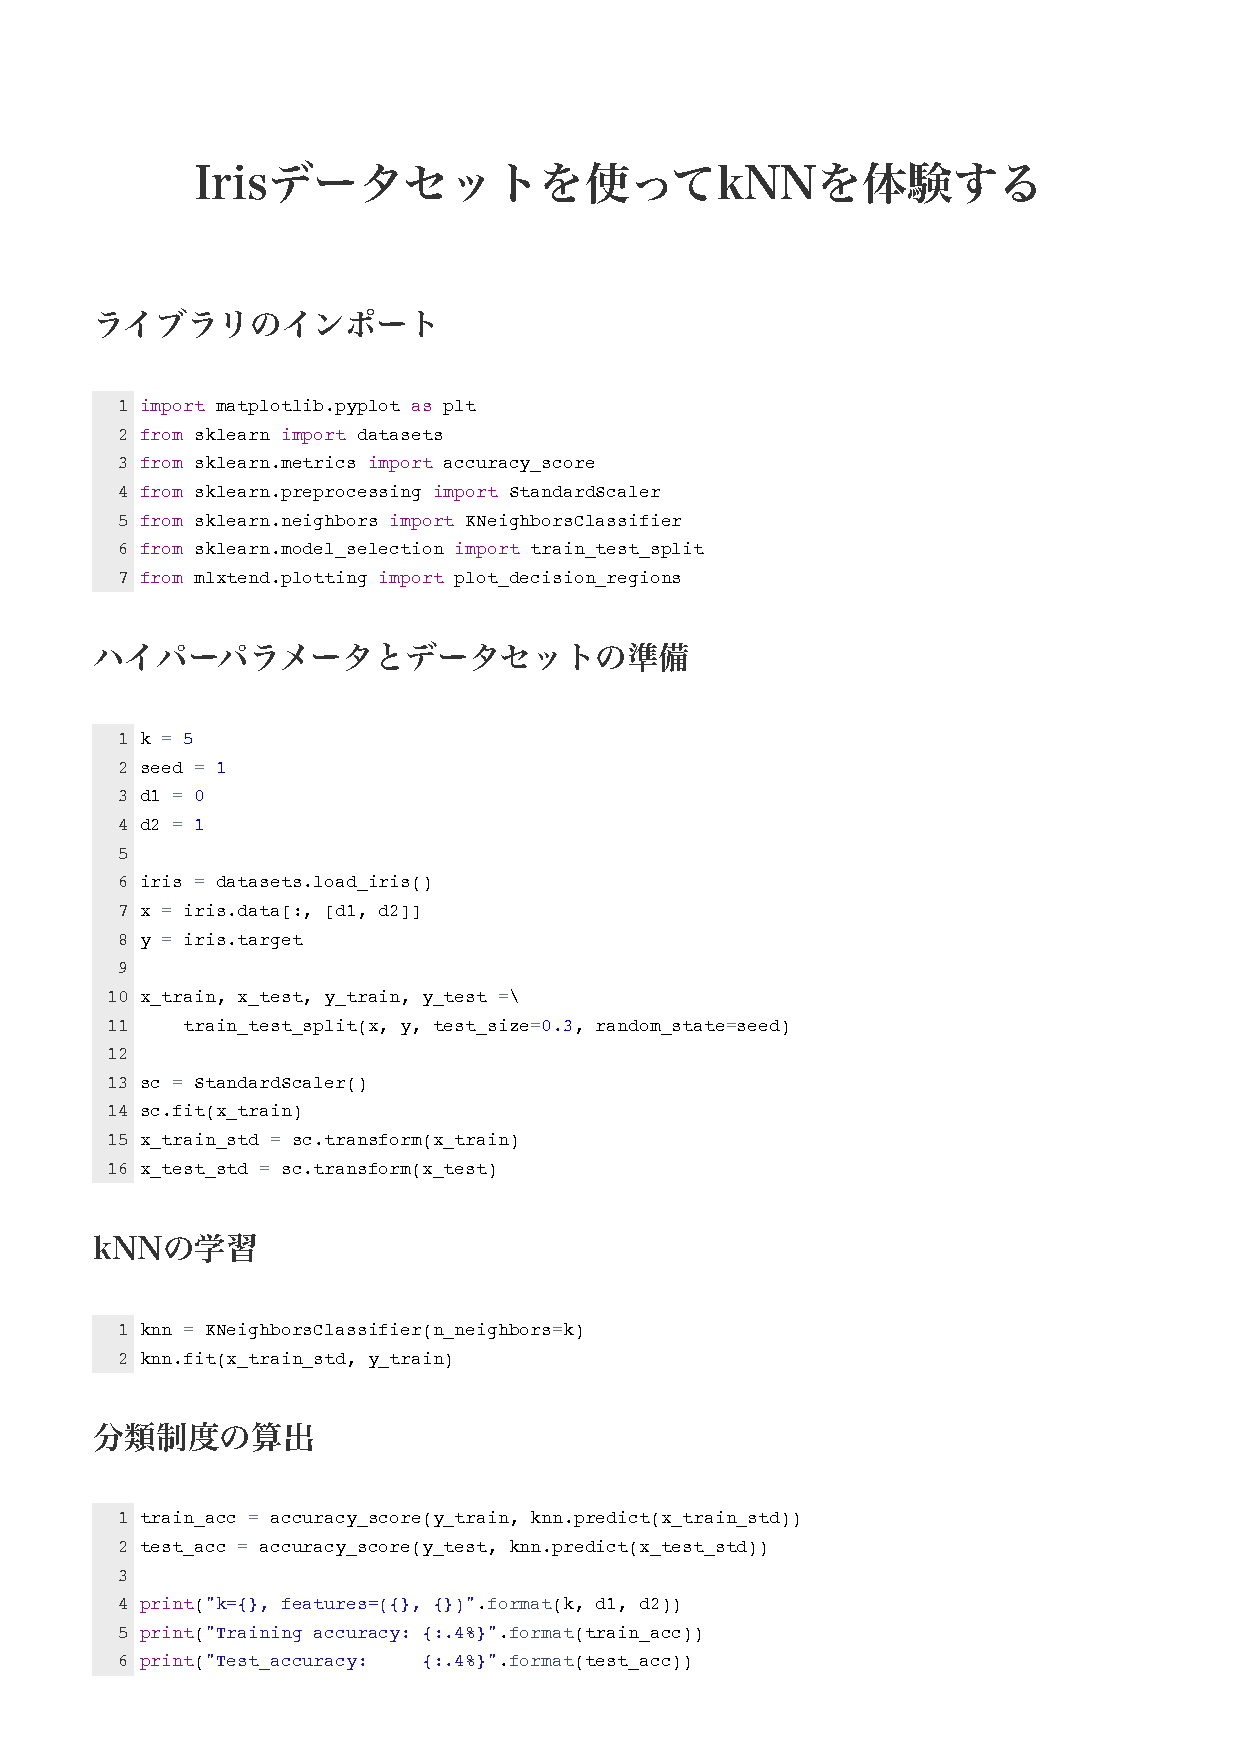
\includepdf[pages=-]{Resources/No1_kNN}
